\documentclass[18pt]{article}

\usepackage[utf8]{inputenc}
\usepackage[T1]{fontenc}
\usepackage{ragged2e}
\usepackage{caladea}
\usepackage{longtable}
\usepackage{wrapfig}
\usepackage{rotating}
\usepackage{epigraph}
\usepackage[normalem]{ulem}
\usepackage{hyperref}
\usepackage{amsmath}
\usepackage{amssymb}
\usepackage{capt-of}
\usepackage{fancyhdr}
\usepackage{graphicx}

\makeatletter
\newcommand{\vers@resp@sym}{%
  \raisebox{0.2ex}{\rotatebox[origin=c]{-20}{$\m@th\rceil$}}%
}
\newcommand{\vers@resp}[2]{%
  {\ooalign{%
     \hidewidth\kern#1\vers@resp@sym\hidewidth\cr
     #2\cr
  }}%
}
\DeclareRobustCommand{\versicle}{\vers@resp{-0.1em}{V}}
\DeclareRobustCommand{\response}{\vers@resp{0pt}{R}}
\makeatother

\date{27 de junho}
\author{Adaptado de publicação devocional}

\renewcommand{\contentsname}{Sumário}

\begin{document}

\tableofcontents

\thispagestyle{empty}
\pagestyle{fancy}
\fancyhf{}
\fancyfoot[LO, CE]{
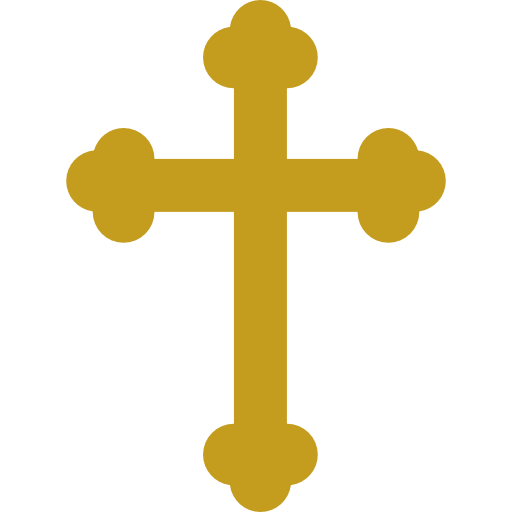
\includegraphics[scale=0.2]{./assets/cross.png} São Cirilo de Alexandria, rogai por nós!
}
\fancyfoot[R]{\thepage}

\centering

\newpage

\section{Introdução}
\begin{justify}
São Cirilo de Alexandria nasceu em 376, em meio às disputas teológicas e políticas que marcavam o fim do Império Romano. Criado sob a tutela de seu tio Teófilo, patriarca de Alexandria, recebeu educação clássica e formação teológica sólidas, mas seus primeiros anos permanecem envoltos em mistério. Ordenado sacerdote por Teófilo, acompanhou-o em 403 ao Sínodo dos Carvalhos, em Constantinopla, que resultou na deposição de São João Crisóstomo.

Em 412, após a morte de Teófilo, Cirilo foi nomeado patriarca de Alexandria em meio a tumultos civis e disputas pelo poder. Dedicou-se a combater a seita dos noviços, que rejeitava a reintegração dos apóstatas, fechando igrejas e defendendo a disciplina eclesiástica. Enfrentou ainda conflitos com autoridades locais e expulsou judeus cuja conduta ferisse a fé cristã.

O ponto alto de seu episcopado ocorreu em 430, quando se opôs vigorosamente a Nestório, patriarca de Constantinopla, que negava a plena humanidade de Cristo e a maternidade divina de Maria. Convocou sínodos em Roma e em Alexandria, presidiu o Concílio de Éfeso (431) e firmou o dogma de Maria Theotókos. Mesmo deposto e preso por opositores de Nestório, foi absolvido pelos legados papais e restabeleceu a comunhão com a Igreja.

Autor de numerosos tratados sobre a Trindade, a Encarnação e a mariologia, Cirilo combateu heresias como o nestorianismo e o pelagianismo, deixando legado doutrinário que mesmo hoje sustenta a fé católica. Declarado Doutor da Igreja em 1882 por Leão XIII, sua festa é celebrada em 27 de junho. Esta novena convida-nos a implorar sua intercessão, seja por Alexandria, pelos teólogos ou por qualquer intenção conforme a vontade divina.
\end{justify}

\newpage

\section{Oração Inicial}
\begin{justify}
Em nome do Pai, do Filho e do Espírito Santo. Amém.

Senhor Deus, agradecemos pela vida de São Cirilo de Alexandria, que consagrou-se a Ti como sacerdote e bispo, defendendo a verdade com coragem e sabedoria. Por sua intercessão, alcançamos a graça que humildemente Te pedimos: \textit{(intenção)}. Que sejamos firmes na fé, ardentes na caridade e dóceis ao Teu Espírito. Por Cristo, nosso Senhor. Amém.

\vspace{0.5cm}

\noindent
\versicle. São Cirilo de Alexandria,\\
\response. rogai por nós!
\end{justify}

\newpage

\section{Meditações de Cada Dia}

\subsection*{Dia I: Formação e Ordenação}
\begin{justify}
São Cirilo nasceu em 376 e foi educado por seu tio Teófilo, patriarca de Alexandria, nas artes clássicas e na teologia. Sob sua tutela, aprendeu o amor à verdade e ao serviço da Igreja, recebendo a ordenação sacerdotal.

\vspace{0.3cm}
\textit{Pai-nosso, Ave-Maria e Glória.}

\noindent
\versicle. Senhor, dá-nos um coração dócil,\\
\response. para aprender Teus mistérios.

\textit{Reza-se a \nameref{sec:OraçãoFinal}}
\end{justify}

\subsection*{Dia II: Sínodo dos Carvalhos}
\begin{justify}
Acompanhou Teófilo ao Sínodo dos Carvalhos, em Constantinopla (403), que depôs São João Crisóstomo. Cirilo, fiel à autoridade da Igreja, reconheceu a justiça daquele julgamento.

\vspace{0.3cm}
\textit{Pai-nosso, Ave-Maria e Glória.}

\noindent
\versicle. Senhor, fortalece-nos na fidelidade,\\
\response. para discernir a Tua vontade.

\textit{Reza-se a \nameref{sec:OraçãoFinal}}
\end{justify}

\subsection*{Dia III: Patriarca em Tempos de Revolta}
\begin{justify}
Em 412, após a morte de Teófilo, tumultos eclodiram em Alexandria entre partidários de Cirilo e de Timóteo. Nomeado patriarca, Cirilo assumiu com coragem o governo da Igreja em meio às controvérsias.

\vspace{0.3cm}
\textit{Pai-nosso, Ave-Maria e Glória.}

\noindent
\versicle. Senhor, concede-nos coragem,\\
\response. para servir-Te em meio às provas.

\textit{Reza-se a \nameref{sec:OraçãoFinal}}
\end{justify}

\subsection*{Dia IV: Combate aos Noviços e Distúrbios}
\begin{justify}
Parte de seu primeiro ministério foi combater a seita dos noviços, que não readmitia apóstatas. Fechou suas igrejas, expulsou os judeus e denunciou ações do governador contrárias à fé.

\vspace{0.3cm}
\textit{Pai-nosso, Ave-Maria e Glória.}

\noindent
\versicle. Senhor, dá-nos zelo,\\
\response. para defender Tua Igreja.

\textit{Reza-se a \nameref{sec:OraçãoFinal}}
\end{justify}

\subsection*{Dia V: Defensor da Mãe de Deus}
\begin{justify}
Em 430, contrapunha-se a Nestório, que negava a plena humanidade de Cristo e a maternidade divina de Maria. Convocou sínodos em Roma e em Alexandria, presidiu Éfeso (431) e confirmou o título Theotókos.

\vspace{0.3cm}
\textit{Pai-nosso, Ave-Maria e Glória.}

\noindent
\versicle. Senhor, ensina-nos a verdade,\\
\response. para honrar Tua Mãe.

\textit{Reza-se a \nameref{sec:OraçãoFinal}}
\end{justify}

\subsection*{Dia VI: Prisão e Liberação}
\begin{justify}
Deposto pelos seguidores de Nestório, foi preso junto com seu adversário. Demonstrada sua inocência pelos legados papais, foi libertado e reconciliou-se com o arcebispo de Antioquia.

\vspace{0.3cm}
\textit{Pai-nosso, Ave-Maria e Glória.}

\noindent
\versicle. Senhor, concede-nos tua paz,\\
\response. para perdoar e reconciliar.

\textit{Reza-se a \nameref{sec:OraçãoFinal}}
\end{justify}

\subsection*{Dia VII: Autor Teológico}
\begin{justify}
Escreveu tratados sobre a Trindade e a Encarnação, combatendo o nestorianismo e o pelagianismo. Seus escritos fortaleceram a ortodoxia e enriqueceram o patrimônio doutrinário da Igreja.

\vspace{0.3cm}
\textit{Pai-nosso, Ave-Maria e Glória.}

\noindent
\versicle. Senhor, dá-nos sabedoria,\\
\response. para compreender Teus mistérios.

\textit{Reza-se a \nameref{sec:OraçãoFinal}}
\end{justify}

\subsection*{Dia VIII: Doutor da Igreja e Mariologia}
\begin{justify}
Em 1882, o Papa Leão XIII declarou-o Doutor da Igreja, destacando sua mariologia e a defesa de Maria como Theotókos, Mãe de Deus, confirmando o amor a Cristo e à Igreja.

\vspace{0.3cm}
\textit{Pai-nosso, Ave-Maria e Glória.}

\noindent
\versicle. Senhor, inflama-nos em amor,\\
\response. por Tua Mãe e por Tua Igreja.

\textit{Reza-se a \nameref{sec:OraçãoFinal}}
\end{justify}

\subsection*{Dia IX: Intercessor de Alexandria e dos Teólogos}
\begin{justify}
Padroeiro de Alexandria, protetor dos governantes e guia dos teólogos, São Cirilo intercede por todos que buscam a verdade e a unidade na fé.

\vspace{0.3cm}
\textit{Pai-nosso, Ave-Maria e Glória.}

\noindent
\versicle. Senhor, atende nossas preces,\\
\response. por intercessão de São Cirilo.

\textit{Reza-se a \nameref{sec:OraçãoFinal}}
\end{justify}

\newpage

\section{Oração Final}
\label{sec:OraçãoFinal}
\begin{justify}
Senhor Deus, que concedestes a São Cirilo de Alexandria sabedoria e coragem para defender a verdadeira fé, concedei também a nós a graça de viver com fidelidade os ensinamentos da vossa Igreja, vencendo todo erro com a luz da vossa verdade. Por sua intercessão, fortalecei-nos na caridade, dai-nos amor à doutrina e zelo pela unidade. Por Cristo, nosso Senhor. Amém.

\vspace{0.5cm}

\noindent
\versicle. São Cirilo de Alexandria,\\
\response. rogai por nós!
\end{justify}

\vfill

Créditos: Adaptado e traduzido de publicação devocional internacional, Disponível em: \url{https://larutadelavirgendeguadalupe.com/novena-a-san-cirilo-de-alejandria/}

\end{document}
